OpenHubo\cite{dlofaro-srm} is an open-source kinematic and dynamic simulator for the the Hubo2 and Hubo2+ series robots.
It was developed by the Drexel Autonomous Systems Lab and runs using the open-source robot simulation environment OpenRAVE\cite{diankovThesis}.
Fig.~\ref{fig:openhubo1} shows the OpenHubo model.
Table~\ref{table:huboOpenSensors} shows the spesifications of OpenHubo.


\begin{figure}[thpb]
  \centering
      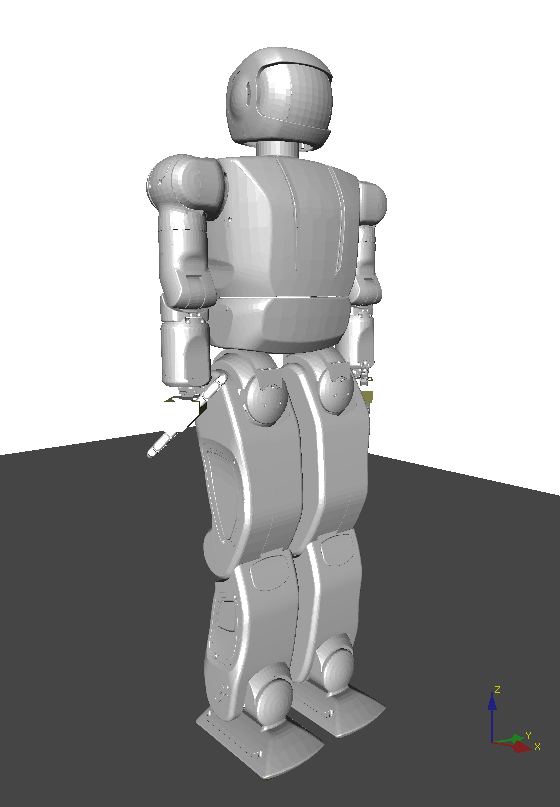
\includegraphics[width=0.4\columnwidth]{./pix/hBody.png}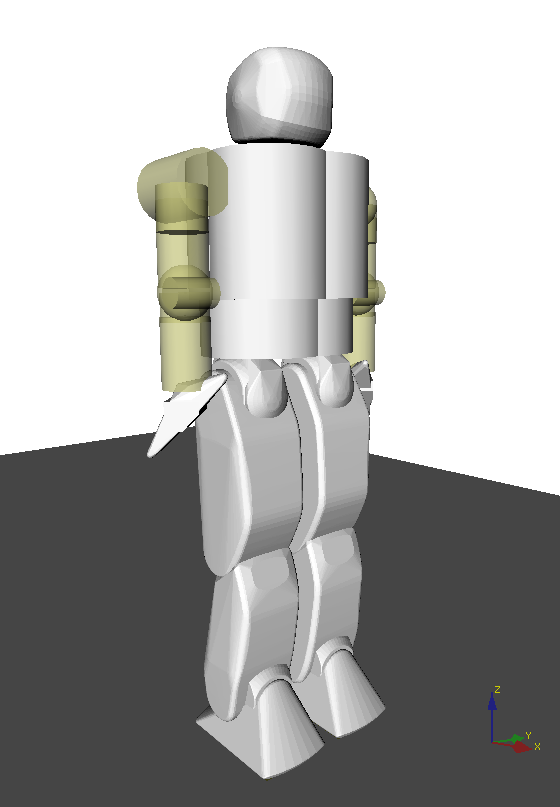
\includegraphics[width=0.4\columnwidth]{./pix/hCol.png}
      
\caption{OpenHubo model of the Hubo2 humanoid robot developed by the Drexel Autonomous Systems Lab and runs using the open-source robot simulation environment OpenRAVE\cite{diankovThesis}.}
\label{fig:openhubo1}
\end{figure}


\begin{table}
\centering
\caption{OpenHubo Platform Specifications}
\begin{tabular}{| l || l |}
\hline
Dynamics      		& Yes (ODE)			\\
\hline
Kinematic		& Yes				\\
\hline
DOF			& 40				\\
\hline
Joint Control Type	& PID Position			\\
\hline
Computer		& $1.6~Ghz$ Atom		\\
			& $2~Gb$ DDR2 RAM		\\
\hline
Enviroment		& OpenRAVE\cite{diankovThesis}	\\

\hline
Sensors			& 1x 4 Axis IMU			\\
			& 4x 3 Axis Force Torque	\\
\hline
\hline
\end{tabular}
\label{table:huboOpenSensors}
\end{table}
